\section{Derivation of the net reproduction rate $ R_0 $ and some of its properties} \label{app::calc_R0}
\begin{refsection}
In this appendix, we derive the net reproduction rate $ R_0(x, \s) $ for a given location $ x $ and a canopy height $ \s $. Finally, we prove that $ R_0(x, \s) $ is a decreasing function of $ \s $ which allows us to make our interpretation in the results section. We suppose that the dispersal kernel $ \K $ is a Dirac, in other words, seeds emitted from $ x $ remain in their source patch $ x $.

\subsection{Derivation of $ R_0 $ \label{calc_R0::sec::R0}}
We use the method of characteristics in equation \eqref{eq::dynamics_x}. This method is commonly used in transport equations, like \eqref{eq::dynamics_x} describing the advection of trees at a non-constant speed  $ G $ along the size axis. Characteristics allow us to follow individuals through their life, \ie they represent the trajectories of individuals in the time-size plan (fig. \ref{fig::chara} for an example). Our transport equation requires an initial population at time $ t = 0 $ that we denote by $ \phi(s) $. It is the density of trees of size $ s $ at the beginning.

\begin{figure}[h!]
	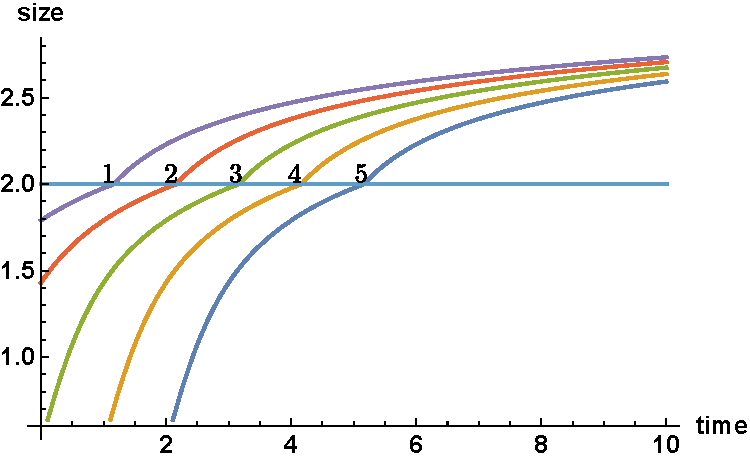
\includegraphics{illustrations/chara}
	\caption{Characteristics for a constant competition $ \s_c = 2 $, a climatic constant $ \xi_{x, i} = 1 $, and for coefficients $ \beta_0 = \ln(3) $, $ \beta_1 = 1 $ and $ \beta_2 = -1 $. These curves are parameterised by $ \theta $ and allow us to follow a cohort with relative time $ \theta $}
	\label{fig::chara}
\end{figure}

Let the canopy height $ \s $ be known with a constant value $ \s_c $, and, let $ s $ and $ t $ be functions of a parameter $ \theta $. By applying the chain rule, we get:
\[
	\frac{d N\big(s(\theta), t(\theta) \big)}{d \theta} = \left. \frac{\partial N}{\partial s} \right|_{(s(\theta), t(\theta))} \frac{ds}{d \theta} +
			\left. \frac{\partial N}{\partial t} \right|_{(s(\theta), t(\theta))} \frac{dt}{d \theta}
\]
We therefore set the characteristic equations to:
% \begin{align}
% 	\frac{ds}{d \theta} &= G(s, \s_c) \label{eq::chara_s} \\
% 		&= \xi_{x, i}(s, \s_c) \exp\left[ -\frac{1}{2} \left( \frac{\ln(s/\phi_{opt})}{\sigma} \right)^2 \right] \nonumber \\
% 	\frac{dt}{d \theta} &= 1 \label{eq::chara_t}
% \end{align}
\begin{align}
	\frac{ds}{d \theta} &= G(s, \s_c) \label{eq::chara_s} \\
		&= \xi_{x, i} e^{\beta_0 \mathbb{1}_{[\s_c, \infty[}(s) + \beta_1 s + \beta_2 s^2} \nonumber \\
	\frac{dt}{d \theta} &= 1 \label{eq::chara_t}
\end{align}
where $ \xi_{x, i} $ is a species-specific ($ i $ index) constant depending of the climate at the location $ x $, and $ \mathbb{1}_A $ is the indicator function (\ie $ \mathbb{1}_A (s) $ equals 1 if $ s \in A $ and 0 otherwise). Hence, equation \eqref{eq::dynamics_x} is along the characteristics:
\begin{equation}
	\frac{dN}{d\theta} = - \left\{ \frac{\partial G}{\partial s}(s, \s, x) + \mu(s, \s, x) \right\} N(\theta) \label{eq::ODE_N}
\end{equation}
\begin{nota}[Abusing notations]
	I am abusing the notations $ N(\theta) $ and $ N\big( s(\theta), t(\theta) \big) $ to make equations easier to read. It would have been more correct to write
	\[
		\widetilde{N}(\theta) = N \big(s(\theta), t(\theta) \big)
	\]
\end{nota}

For the sake of readability, I drop the $ x $ in $ G $ and $ \mu $, and write $ \exp $ for the exponential function instead of $ e^x $. The solution of \eqref{eq::ODE_N} is:
\begin{equation} \label{eq::sol_ODE_N}
	N(\theta_1) = N(\theta = 0) \exp \left[-\int_0^{\theta_1} \mu(s, \s_c) + \frac{\partial G}{\partial s}(s, \s_c) \, d\theta \right]
\end{equation}
where the boundary condition $ N(\theta = 0) = N(s_{\theta = 0}, t_{\theta = 0}) $, and the coordinates $ (s(\theta_1), t(\theta_1)) $ are to be determined. We denoted $ s_{\theta = 0} $ to specify it is the origin of the characteristic but still distinguish it from $ s_0 $, the size of newborns. The time coordinate, solution of \eqref{eq::chara_t}, is denoted by $ T $:
\[
	T(\theta) = \theta + t_{\theta = 0}
\]
however, the $ i $-state coordinate $ s $ cannot be expressed in terms of elementary functions. In what follows, we assume $ \beta_2 < 0 $ which is true for all the species we parameterised. Thus, the integral
\begin{align*}
	\int  | G(s, \s_c) | \, ds &\leqslant \int e^{|\beta_0|} e^{\beta_1 s + \beta_2 s^2} \, ds \\
	&\leqslant e^{|\beta_0| - \frac{\beta_1^2}{4 \beta_2^2}} \int e^{\beta_2(s + \sfrac{\beta_1}{2\beta_2})^2} \, ds
\end{align*}
exists and equation \eqref{eq::chara_s} has a solution that we denote by $ S(\theta_1, s_{\theta = 0}, \s_c) $. This solution $ S(\theta_1, s_{\theta = 0}, \s_c) $ is the coordinate of the $ i $-state at $ \theta_1 $ along the characteristic originated in $ s_{\theta = 0} $ at $ t_{\theta = 0} $.

Let us assume that $ S $ admits an inverse, in other words, there exists a function $ \tau $ such that:
\begin{align*}
	\tau \big( S(\theta_1, s_{\theta = 0}, \s_c), s_{\theta = 0}, \s_c \big) &= \theta_1 \\
	S \big(\tau(s_1, s_{\theta = 0}, \s_c), s_{\theta = 0}, \s_c \big) &= s_1
\end{align*}
In other words, $ \tau(s_1, s_0, \s_c) $ is the time it requires to grow from $ s_0 $ to $ s_1 $ under competition $ \s_c $. Although, equation \eqref{eq::dynamics_x} cannot be solved analytically (we would need an explicit solution of $ S $ and $ \tau $), the net reproduction rate is still tractable. Indeed, equation \eqref{eq::sol_ODE_N} can be rewritten:
\begin{align*}
	N \big( s(\theta_1), t(\theta_1) \big) &= N( s_{\theta = 0}, t_{\theta = 0}) \exp \left[-\int_0^{\theta_1} \mu(s, \s_c) + \frac{\partial G}{\partial s}(s, \s_c) \, d\theta \right] \\
	&= N( s_{\theta = 0}, t_{\theta = 0}) \exp \left[-\int_{s_{\theta = 0}}^{s(\theta_1)} \left( \mu(s, \s_c) + \frac{\partial G}{\partial s}(s, \s_c) \right) \frac{d \theta}{ds} \, ds \right] \\
	&= N( s_{\theta = 0}, t_{\theta = 0}) \exp \left[-\int_{s_{\theta = 0}}^{s(\theta_1)} \left( \mu(s, \s_c) + \frac{\partial G}{\partial s}(s, \s_c) \right) \frac{1}{G(s, \s_c)} \, ds \right] \\
	&= N( s_{\theta = 0}, t_{\theta = 0}) \frac{G(s_{\theta = 0}, \s_c)}{G \big( s(\theta_1), \s_c \big)} \exp \left[-\int_{s_{\theta = 0}}^{s(\theta_1)} \frac{\mu(s, \s_c)}{G(s, \s_c)} \, ds \right] \\
\end{align*}

If a characteristic emerged at $ t_{\theta = 0} \leqslant 0 $, then it concerns the initial population (at $ t = 0 $) denoted by $ \phi(s) $:
\begin{equation}\label{eq::sol_init}
	N(S(t, s, \s_c), t) = \phi(s) \frac{G(s, \s_c)}{G\big( S(t, s, \s_c), \s_c \big)} \exp \left[ -\int_{s}^{S(t, s, \s_c)} \frac{\mu(\sigma, \s_c)}{G(\sigma, \s_c)} \, d\sigma \right]
\end{equation}
where $ S(t, s, \s_c) $ is the size of the individual at time $ t $ given at time $ 0 $ they were of size $ s $. In figure \ref{fig::chara}, the characteristics that emerged before $ t = 0 $ are the first, second and third curves.

For characteristics that emerged after time 0 (fourth and fifth curves on fig \ref{fig::chara}), we denote their birth coordinates $ (s_{\theta = 0}, t_{\theta = 0}) $ by $ (0, t_b) $; $ t_b > 0 $ stands for the time of birth.
\begin{equation}\label{eq::sol_later}
	N(s, t) = N \big( 0, t - \tau(s, 0, \s_c) \big) \frac{G(0, \s_c)}{G(s, \s_c)} \exp \left[ -\int_{0}^{s} \frac{\mu(\sigma, \s_c)}{G(\sigma, \s_c)} \, d\sigma \right]
\end{equation}

The initial population (equation \eqref{eq::sol_init}) goes extinct as $ t $ goes by. Therefore, only equation \eqref{eq::sol_later} is of interest \citep{DeRoos1997}. We now use the boundary condition \eqref{eq::recruitment_x} (once again, we drop the spatial variable $ x $ since the dispersal kernel $ \K $ is a Dirac):
\begin{align*}
	N(0, t) G(0, \s_c) &= \int_{0}^{\infty} F(s, \s_c) N(s, t) \, ds \\
		&= \int_{0}^{\infty} F(s, \s_c) N \big( 0, t - \tau(s, 0, \s_c) \big) \frac{G(0, \s_c)}{G(s, \s_c)} \exp \left[ -\int_{0}^{s} \frac{\mu(\sigma, \s_c)}{G(\sigma, \s_c)} \, d\sigma \right] \, ds
\end{align*}
Let
\[
	B(t, \s_c) = N(0, t) G(0, \s_c)
\]
the population birth rate (\ie the quantity of seedlings created at time $ t $ by a population undergoing a competition $ \s_c $). We can substitute $ B $ into the previous equation:
\begin{equation} \label{eq::popBirth}
	B(t, \s_c) = \int_{0}^{\infty} B \big(t - \tau(s, 0, \s_c), \s_c \big) \frac{F(s, \s_c)}{G(s, \s_c)} \exp \left[ -\int_{0}^{s} \frac{\mu(\sigma, \s_c)}{G(\sigma, \s_c)} \, d\sigma \right] \, ds
\end{equation}
If $ \tau $ were a known function (which is not the case here), equation \eqref{eq::popBirth} would relate the population birth rate to its past. The quantity
\[
	\frac{1}{G(s, \s_c)} B \big(t - \tau(s, 0, \s_c), \s_c \big) \exp \left[ -\int_{0}^{s} \frac{\mu(\sigma, \s_c)}{G(\sigma, \s_c)} \, d\sigma \right]
\]
is just the density of individuals born $ t - \tau $ times unit ago that survived up to a size in $ [s, s + ds] $ at time $ t $, and $ B $ is the `input flow' per unit time.

Equation \eqref{eq::popBirth} admits an equilibrium only for particular combinations of parameters $ G $, $ \mu $ and $ F $ and since there is no density dependence here ($ \s $ is set to a known value $ \s_c $), then $ B $ ultimately grows or decline exponentially \citep{DeRoos1997}. We therefore substitute the trial solution
\begin{equation} \label{eq::B_trial}
	B(t, \s_c) = B_0e^{\lambda t}
\end{equation}
into \eqref{eq::popBirth} to get:
\begin{align*}
	B_0 e^{\lambda t} &= \int_{0}^{\infty} B_0 e^{\lambda t - \lambda \tau(s, 0, \s_c)} \frac{F(s, \s_c)}{G(s, \s_c)} \exp \left[ -\int_{0}^{s} \frac{\mu(\sigma, \s_c)}{G(\sigma, \s_c)} \, d\sigma \right] \, ds \\
	&= B_0 e^{\lambda t} \int_{0}^{\infty} e^{- \lambda \tau(s, 0, \s_c)} \frac{F(s, \s_c)}{G(s, \s_c)} \exp \left[ -\int_{0}^{s} \frac{\mu(\sigma, \s_c)}{G(\sigma, \s_c)} \, d\sigma \right] \, ds \\
\end{align*}
Thus, we get:
\begin{equation} \label{eq::eigen}
	1 = \int_{0}^{\infty} e^{- \lambda \tau(s, 0, \s_c)} \frac{F(s, \s_c)}{G(s, \s_c)} \exp \left[ -\int_{0}^{s} \frac{\mu(\sigma, \s_c)}{G(\sigma, \s_c)} \, d\sigma \right] \, ds
\end{equation}
When $ \lambda $ is setted to 0, the right hand side of \eqref{eq::eigen} becomes:
\begin{equation} \label{eq::R0_app}
	\int_{0}^{\infty} \frac{F(s, \s_c)}{G(s, \s_c)} \exp \left[ -\int_{0}^{s} \frac{\mu(\sigma, \s_c)}{G(\sigma, \s_c)} \, d\sigma \right] \, ds
\end{equation}
It represents the expected number of seedlings produced by an individual through its lifespan, which is by definition the net reproduction rate $ R_0(\s_c) $ we were looking for (equation \eqref{eq::R0sol}). Given only canopy individuals can reproduce, $ \forall s < \s_c $, $ F(s, \s_c) = 0 $ and $ \forall s \geqslant \s_c $, $ F(s, \s_c) > 0 $ and therefore the lower limit of the integrals can be changed to $ \s_c $ in equation \eqref{eq::R0_app}:
\[
	R_0 = \exp \left[- \int_{0}^{\s_c} \frac{\mu(\sigma, \s_c)}{G(\sigma, \s_c)} \, d\sigma \right] \times \int_{\s_c}^{\infty} \frac{F(s, \s_c)}{G(s, \s_c)} \exp \left[ - \int_{\s_c}^{s} \frac{\mu(\sigma, \s_c)}{G(\sigma, \s_c)} \, d\sigma \right] \, ds
\]
\begin{rem}[On $ \lambda $]
	If $ \lambda = 0 $ is truly solution of \eqref{eq::eigen}, then $ R_0(\s_c) = 1 $ and the population is stable. This is consistent with \eqref{eq::B_trial} since in this case the population birth rate would be constant.
\end{rem}

The constant $ \lambda $ is called the intrinsic growth rate of the population. Let us now prove that $ \lambda > 0 $ is equivalent to a net reproduction rate $ R_0(\s_c) > 1 $. Denote by $ f $ the function:
\[
	f(\lambda) = \int_{0}^{\infty} e^{- \lambda \tau(s, 0, \s_c)} \frac{F(s, \s_c)}{G(s, \s_c)} \exp \left[ -\int_{0}^{s} \frac{\mu(\sigma, \s_c)}{G(\sigma, \s_c)} \, d\sigma \right] \, ds
\]
We have:
\begin{align*}
	f'(\lambda) &= -\lambda f(\lambda) \\
	f''(\lambda) &= +\lambda^2 f(\lambda)
\end{align*}
Given $ f $ is a positive function (fecundity and growth are positive functions), then $ f $ is a convex decreasing function on $ \R^{+} $ and its maximum is reached at $ \lambda = 0 $. Hence, if $ R_0 > 1 $:
\[
	f(\lambda) = 1
\]
admits a unique solution on $ \R^{+} $. Thus
\[
	R_0 > 1 \Leftrightarrow \lambda > 0
\]

\subsection{Proofs of the three assertions \label{app::calc_R0::sec::3asser}}
We now prove the three following assertions:
\begin{enumerate}[label=(\textit{\roman*})]
	\item $ R_0(\s_c) $ is a decreasing function
	\item $ R_0 $ is an increasing function of the average understorey growth $ \bar{G} $ and a decreasing function of the average mortality $ \bar{\mu} $
	\item $ R_0 $ is an increasing function of the average fecundity $ \bar{F} $
\end{enumerate}

\subsubsection{First assertion}
The easiest argument to prove $ R_0 $ is a decreasing function of $ \s $ is to see that all the integrand's parts are always positive. Let:
\[
	f(s_1) = \int_{s_1}^{\infty} \frac{F}{G} e^{-\int_{s_1}^s \frac{\mu}{G} \, d\sigma} \, ds
\]
For any $ s_1 \leqslant s_2 $ we have:
\begin{align*}
	R_0(s_1) - R_0(s_2) &= e^{-\int_{0}^{s_1} \frac{\mu}{G} \, ds} \left[ \left( 1 - e^{-\int_{s_1}^{s_2} \frac{\mu}{G} \, ds} \right) f(s_2) + \int_{s_1}^{s_2} \frac{\mu}{G} \, ds \right] \\
		&\geqslant 0
\end{align*}
Therefore, $ R_0 $ is a decreasing function of $ \s $.

\subsubsection{Second assertion}
The average understorey growth for a canopy height $ \s $ is defined by
\[
	\bar{G} = \frac{1}{\s} \int_0^{\s} G(s, \s) \, ds
\]
Let $ G_1 $ and $ G_2 $ two growth functions. Since the overstorey growth is not changed, we just study the ratio:
\begin{equation} \label{eq::ratio_G}
	\frac{e^{\int_0^{\s} \frac{\mu}{G_1} \, ds}}{\int_0^{\s}e^{\frac{\mu}{G_2} \, ds}}
\end{equation}
We want to find a sufficient condition on $ G_1 $ and $ G_2 $ to get this ratio larger than 1, which means the net reproduction rate $ R_0 $ increases. Equation \eqref{eq::ratio_G} can be be rewritten:
\[
	e^{\int_0^{\s} \frac{\mu (G_1 - G_2)}{G_1 G_2} \, ds} \geqslant 1 \quad \Leftrightarrow \quad \int_0^{\s} \frac{\mu (G_1 - G_2)}{G_1 G_2} \, ds \geqslant 0
\]
Given $ \mu $ and $ G $ are positive functions, we can lower bound the integrand:
\begin{equation} \label{eq::minor}
	\frac{\mu (G_1 - G_2)}{G_1 G_2} \geqslant \frac{\max(\mu)}{\min(G_1 G_2)} \mathds{1}_{G_1 < G_2} (s) \times (G_1 - G_2) + \frac{\min(\mu)}{\max(G_1 G_2)} \mathds{1}_{G_1 \geqslant G_2}(s) \times (G_1 - G_2)
\end{equation}
Define
\[
	\begin{matrix}
		k_1 = \frac{\max(\mu)}{\min(G_1 G_2)} & &
			\mathscr{D}_1 = \{ s | G_1(s) < G_2(s) \} \\
		k_2 = \frac{\min(\mu)}{\max(G_1 G_2)} & &
		 	\mathscr{D}_2 = \{ s | G_1(s) \geqslant G_2(s) \}\\
	\end{matrix}
\]
equation \eqref{eq::minor} is:
\begin{align*}
	\int_0^{\s} \frac{\mu (G_1 - G_2)}{G_1 G_2} &\geqslant
		k_1 \int_{\mathscr{D}_1} G_1  \, ds + k_2 \int_{\mathscr{D}_2} G_1 \, ds +
		k_1 \int_{\mathscr{D}_1} G_2  \, ds + k_2 \int_{\mathscr{D}_2} G_2 \, ds \\
	&\geqslant \min (k_1, k_2) \left[\int_{\mathscr{D}_1 \cup \mathscr{D}_2} G_1 \, ds + \int_{\mathscr{D}_1 \cup \mathscr{D}_2} G_2 \, ds \right]
\end{align*}
Therefore, given $ \mathscr{D}_1 \cup \mathscr{D}_2 = [0, \s] $, a sufficient condition to have the ratio defined by equation \eqref{eq::ratio_G} larger than $ 1 $ is:
\begin{equation}
	\int_0^{\s} G_1 \, ds \geqslant \int_0^{\s} G_2 \, ds,
\end{equation}
that is to say:
\[
	\bar{G}_1 \geqslant \bar{G}_2
\]
Thus, when the understorey growth increases in average, so does the net reproduction rate $ R_0 $. A similar reasoning on $ \mu $ would prove that increasing the understorey mortality induce a depleted $ R_0 $. This conclude the proof of the second assertion.

\subsubsection{Third assertion}
In this article, we used the fecundity of \citet{Purves2008} which is proportional to sun-exposed crown area $ \A $:
\[
	F(s, \s) = f \A(s, \s)
\]
where $ f $ is the new recruits per unit time per crown area.
\begin{align*}
	\frac{\partial R_0}{\partial f} &= e^{-\int_0^{\s} \frac{\mu}{G} \, ds} \int_{\s}^{\infty} \frac{A}{G} e^{-\int_{\s}^{s} \frac{\mu}{G} \, d \sigma} \, ds \\
		&\geqslant 0
\end{align*}
Thus, increasing fecundity augments $ R_0 $, which proves the third assertion.

\printbibliography[heading=subbibliography]
\end{refsection}
